\chapter{Введение}

\section{Формула интегрирования по частям}

Возьмём ограниченную область $ \Omega \sub \R^n $.
$ \partial \Omega $ "--- кусочно-гладкая.
Рассмотрим вектор-функцию $ f : \ol \Omega \to \R^n $.
Считаем, что $ f \in \mathcal C^1 $.
Тогда справедлива формула Гаусса"--~Остроградского:
$$ \int\limits_\Omega \dive(f) \di x = \int\limits_{\partial \Omega} (f, \vv n) \di S $$
Будем всегда считать, что $ \vv n $ "--- внешняя нормаль.

\begin{definition}
	$$ \dive(f) = \sum_i \frac{\partial f_i}{\partial x_i} $$
	(если не пишем пределы суммирования, то по-умолчанию считается, что суммируем от 1 до $ n $).
\end{definition}

Рассмотрим $ f = uve_k $, где $ u, v \in \mathcal C^1 $, $ e_k $ "--- $ k $-й орт стандартного
базиса.

$$ \int\limits_\Omega \frac{\partial(uv)}{\partial x_k} \di x =
\int\limits_{\partial \Omega} uv \vv n_k \di S $$
Получаем \emph{формулу интегрирования по частям:}
$$ \int\limits_\Omega \frac{\partial u}{\partial x_i} v \di x =
\int\limits_{\partial \Omega} uv \vv n_k \di S -
\int\limits_\Omega u \frac{\partial v}{\partial x_i} \di x $$

\chapter{Вывод основных уравнений математической физики}

\section{Уравнение теплопроводности (heat equation)}

\begin{problem}
	Есть какое-то тело, в нём происходят какие-то процессы.
	Возьмём в теле кусочек $ G $ с кусочно-гладкой границей.
	Какое количество теплоты $ Q $ в этом кусочке содержится (как оно изменяется в течение
	промежутка времени $ [t_1, t_2] $)?
\end{problem}

Обозначим $ Q_1 $ "--- количество теплоты, которое \emph{выделилось} в $ G $ на отрезке $ [t_1, t_2] $.
При этом, из него \emph{вытекло} $ Q_2 $ теплоты.
Есть закон сохранения теплоты:
$$ Q_1 - Q_2 = Q $$

Пусть процесс описывается функцией $ F(x, t) $, где $ x $ "--- точка в пространстве,
$ t $ "--- время.
$ F $ "--- \emph{плотность мощности источников тепла}.

$$ Q_1 = \int_{t_1}^{t_2} \int\limits_G F(x, t) \di x \di t = Q_1 $$
$$ Q_2 = \int_{t_1}^{t_2} \int\limits_{\partial G} \di \Phi \di t $$
$ \Phi $ "--- плотность потока тепла в единицу времени.

Если $ U(x, t) $ "--- температура, то
$$ -\mathcal D U = -\Bigl( \frac{\partial u}{\partial x_1}, \dots, \frac{\partial u}{\partial x_n} \Bigr) $$
$ -\mathcal D U $ "--- направление наискорейшего убывания температуры.
Возьмём вектор, ему пропорциональный:
$$ -k(x) \mathcal DU $$

$$ \di \Phi = -k(x) (\mathcal D U, \vv n) \di S $$

$$ Q_2 = \int_{t_1}^{t_2} \int\limits_{\partial G} -k(x) (\mathcal D U, \vv n) \di S \di t $$

Обозначим $ c(x) $ "--- \emph{удельная теплоёмкость}, $ \rho(x) $ "--- \emph{плотность}.

$$ \int\limits_G \bigl( U(x, t_2) - U(x, t_1) \bigr) c(x) \rho(x) \di x = Q $$

Хотим подставить всё это в уравнение теплового баланса.
Но пределы у интегралов разные, поэтому сначала нужно привести интегралы к единому виду.

$$ Q_2 = \int_{t_1}^{t_2} \int\limits_G \dive (-k \mathcal D U) \di x \di t $$
$$ Q = \int_{t_1}^{t_2} \int\limits_G \frac{\partial U}{\partial t} c(x) \rho(x) \di x \di t $$

$$ \int_{t_1}^{t_2} \int\limits_G \Bigl( c \rho \frac{\partial U}{\partial t} -
\dive (k \mathcal D U) - D \Bigr) \di x \di t = 0 $$
(конечно же, мы предполагали, что все нужные нам функции достаточно гладкие)

Получили \emph{уравнение теплопроводности}:
$$ c(x) \rho(x) \frac{\partial U}{\partial t} - \dive \bigl( k(x) \mathcal D U \bigr) = F(x, t) $$
Считаем тело изотропным.
Если бы оно было анизотропным, то вместо $ k(x) $ стояла бы матрица $ n \times n $.

Если тело к тому же однородное, то все коэффициенты "--- константы:
$$ \dive (\mathcal D U) =
\sum_i \frac{ \partial \bigl( \frac{\partial U}{\partial x_i} \bigr)}{\partial x_i} =
\sum_i \frac{\partial^2 U}{\partial x_i^2} = \Delta U $$
$ \Delta U $ "--- \emph{оператор Лапласса} от $ U $ (\emph{Лаплассиан}).

Поделим на $ c $ и на $ \rho $:
$$ \frac{\partial U}{\partial t} - a^2 \Delta U = f(x, t) $$
Это уравнение тоже называется \emph{уравнением теплопроводности} (для однородного изотропного тела).

Можно задать \emph{граничные условия}:
\begin{enumerate}
	\item Пусть $ \Gamma_1 $ "--- некий кусок $ \partial \Omega $, на котором поддерживается
		фиксированная температура (не обязательно постоянная, но обязательно известная).
		$$ U \bigr|_{x \in \Gamma_1} = U_1(x, t) $$

		Говорят, что на $ \Gamma_1 $ задано \emph{условие Дирихле}.
	\item $ -k(\mathcal DU, \vv n) \bigr|_{x \in \Gamma_2} = 0 $

		При этом,
		$$ (\mathcal D U, \vv n) = \frac{\partial U}{\partial \vv n} $$

		Если на границе приходит какое-то количество теплоты (например, стоит радиатор), то
		$$ k(\mathcal DU, \vv n) \bigr|_{x \in \Gamma_2} = U_2(x, t) $$
		В таком случае говорят, что на этой части границы задано \emph{условие Неймана}.
	\item Бывают более сложные условия.
\end{enumerate}

Имеем цилиндр $ \Omega \times (0, T] $ (тут бы нарисовать, но это тяжело).

Будем считать, что задано начальное условие: $ U\bigr|_{t = 0} = \phi(x) $.

Итого,
$$
\begin{cases}
	\text{уравнение теплопроводности в } \Omega \times (0, T], \\
	\text{граничные условия на } \partial \Omega \times [0, T], \\
	\text{начальные условия на } \ol \Omega \times \Set{0}.
\end{cases} $$
Этот комплекс именуется \emph{начальной краевой задачей для уравнения теплопроводности}.

\subsection*{Частные случаи}

\begin{enumerate}
	\item $ \Omega = \R^n $
		$$
		\begin{cases}
			U_t' - a^2 \Delta U = f \\
			U \bigr|_{t = 0} = \phi(x)
		\end{cases} $$
		(граничных условий нет)

		Это "--- \emph{задача Коши} для уравнения теплопроводности.
	\item Однажды температура в помещении стабилизируется, и больше зависеть от времени не будет.

		В таком случае можно считать, что функция задана не на цилиндре, а в $ \Omega $.
		$$ -U = \frac{f(x)}{a^2} $$
		Это "--- \emph{уравнение Пуассона}.

		Если $ f = 0 $ и $ \Delta U = 0 $, то такое уравнение называется \emph{уравнением Лапласса}.

		Если к уравнению Пуассона добавить граничные условия, то получим \emph{краевую задачу для
		уравнения Пуассона (Лапласса)}.
\end{enumerate}

\section{Волновое уравнение}

Рассмотрим поперечные колебания мембраны под воздействием некоторых внешних сил.

Зададим \emph{функционал действия}:
$$ S = \int_{t_1}^{t_2} (K - \Pi) \di t, $$
где $ K $ "--- кинетическая энергия, $ \Pi $ "--- потенциальная энергия.

$$ K = \int\limits_\Omega \frac12 \rho(x) \Bigl( \frac{\partial U}{\partial t} \Bigr)^2 \di x $$

Потенциальная энергия, возникающая под воздействием внешних сил:
$$ \Pi_1 = \int\limits_\Omega = -F(x, t) U \di x $$

\begin{figure}[h]
	\centering
	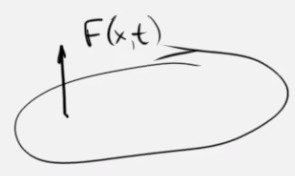
\includegraphics{membrane}
\end{figure}

Потенциальная энергия, возникающая под воздействием упругости мембраны:
$$ \Pi_2 = \int\limits_\Omega k(x) (\di S - \di x) $$
Известно, что $ \di S = \sqrt{1 + |\mathcal D U|^2} \di x $ (это обобщение формулы для длины дуги).
Получаем, что
$$ \Pi_2 = \int\limits_\Omega k(x) \bigl( \sqrt{1 + |\mathcal DU|^2} - 1 \bigr) \di x $$

Будем считать, что мембрана совершает малые колебания.

\begin{definition}
	Будем называть колебания \emph{малыми}, если функция $ U $ и её производная малы настолько, что
	можно пренебречь старшими степенями по сравнению с низкими (то есть, величина мала настолько,
	что уменьшается при увеличении степени).
\end{definition}

Запишем ряд Тейлора:
$$ \sqrt{1 + |\mathcal DU|^2} - 1 \simeq \frac12 |\mathcal D U|^2 $$
(этот значок не опечатка; он означает, что остальными членами можно пренебречь)

Теперь
$$ S = \int_{t_1}^{t_2} \int\limits_\Omega \Bigl\lgroup \frac12 \rho
\Bigl( \frac{\partial U}{\partial t} \Bigr)^2 - \frac12 k \Bigl(
\bigl( \frac{\partial U}{\partial x_1} \bigr)^2 + \bigl( \frac{\partial U}{\partial x_2} \bigr)^2
\Bigr) + FU \Bigr\rgroup \di x \di t $$
Будем считать, что $ U \in \mathcal C^1 \bigl( \ol \Omega \times [t_1, t_2] \Bigr) $.
Пусть известно положение мембраны в начале, в конце, и на некоторой части границы:
$$
\begin{cases}
	U\bigr|_{t = t_1} = U_1(x), \\
	U\bigr|_{t = t_2} = U_2(x), \\
	U\bigr|_{x \in \Gamma_1} = U_3(x, t).
\end{cases} $$

При этом, в некоторых местах стоят планочки, а на них колечки, прикреплённые к мембране.
Получается, что мембрана может двигаться только вертикально, но без трения.

\begin{figure}[h]
	\centering
	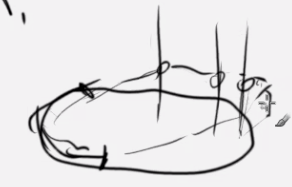
\includegraphics{rings}
\end{figure}

Как известно, для функции нескольких переменных необходимое условие локального экстремума выглядит
так:
$$ \frac{\di S}{\di \alpha}(U + \alpha h) \bigr|_{\alpha = 0} = 0 $$
Посчитаем эту производную:
$$ \Bigl[ \frac12 \rho \Bigl( \frac{\partial U}{\partial t} +
\alpha \frac{\partial h}{\partial t} \Bigr)^2 \Bigr]_\alpha' =
\rho \Bigl( \frac{\partial U}{\partial t} +
\alpha \frac{\partial h}{\partial t} \Bigr) \frac{\partial h}{\partial t} $$

$$ \int_{t_1}^{t_2} \int\limits_\Omega \Bigl\lgroup \rho \frac{\partial U}{\partial t}
\frac{\partial h}{\partial t} - k \Bigl( \frac{\partial U}{\partial x_1}
\frac{\partial h}{\partial x_1} + \frac{\partial U}{\partial x_2}
\frac{\partial h}{\partial x_2} \Bigr) + FU \Bigr\rgroup \di x \di t = 0 $$
Это должно быть выполнено для всех функций
$ h \in \mathcal C^1 \bigl( \ol \Omega \times [t_1, t_2] \bigr) $ таких, что
$$
\begin{cases}
	h\bigr|_{t = t_1} = 0, \\
	h\bigr|_{t = t_2} = 0, \\
	h\bigr|_{x \in \Gamma_1} = 0.
\end{cases} $$

Обозначим цилиндр $ \mathscr C = \Omega \times (t_1, t_2) $.
$$ \int\limits_{\mathscr C} \rho \Bigl( \frac{\partial U}{\partial t}
\frac{\partial h}{\partial t}) \di x \di t =
\underbrace{\int\limits_{\partial \mathscr C} \rho \frac{\partial U}{\partial t} h \vv n_t \di S}_0
- \underbrace{\int\limits_{\mathscr C} \frac{\partial}{\partial t}
\Bigl( \rho \frac{\partial U}{\partial t} \Bigr)h \di x \di t}_{\rho
\frac{\partial^2 U}{\partial t^2}} $$

$$ \int\limits_{\mathscr C} h \Bigl\lgroup -\rho \frac{\partial^2 U}{\partial t^2} +
\frac{\partial}{\partial x_1} \Bigl(k \frac{\partial U}{\partial x_1}\Bigr) +
\frac{\partial}{\partial x_2} \Bigl( k \frac{\partial U}{\partial x_2} \Bigr) + F \Bigr\rgroup
\di x \di t $$

\begin{equ}1
	- \int\limits_{\Gamma_2 \times (t_1, t_2)} h \Bigl( k \frac{\partial U}{\partial x_1} \vv n_1 +
	k \frac{\partial U}{\partial x_2} \vv n_2 \Bigr) \di S = 0
\end{equ}

\subsection(Лемма Дюбуа--Раймона){Лемма Дюбуа"--~Раймона}

\begin{notation}
	$ \mathcal C_0^\infty $ "--- бесконечно гладкие функции с компактным носителем.
\end{notation}

\begin{lemma}
	$ f \in \mathrm L_{1, loc}(\Omega) $ (это означает, что $ \int\limits_K |f| < \infty $ на любом
	компакте $ K \sub \Omega $), $ \quad \Omega \sub \R^n $
	$$ \int\limits_\Omega f(x)h'(x) \di x = 0 \quad \forall h \in \mathcal C_0^\infty(\Omega) $$

	$$ \implies f(x) \equiv 0 \text{ \ale на } \Omega $$
\end{lemma}

\begin{proof}[для $ f \in \mathcal C(\Omega) $]
	Рассмотрим
	$$ \omega_\eps(x) =
	\begin{cases}
		C(\eps) \exp \bigl( \frac1{|x|^2 - \eps^2} \bigr), \quad |x| < \eps, \\
		0
	\end{cases} $$
	$$ \int\limits_{\R^n} \omega_\eps(x) \di x = 1 $$

	\textbf{Предположим}, что $ f(x^0) > 0 $.
	Тогда существует $ x $ такой, что $ f(x) > 0 $ и $ |x - x^0| < \eps $.

	Рассмотрим $ h(x) = \omega_\eps (x - x^0) $.
	Понятно, что $ h(x) \in \mathcal C_0^\infty (\Omega) $.
\end{proof}

\begin{figure}[h]
	\centering
	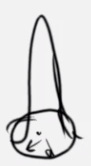
\includegraphics{omega}
	\caption{$ \omega_\eps(x) $}
\end{figure}

$$ -\rho \frac{\partial^2 U}{\partial t^2} + \dive (k \mathcal D U) + F = 0 $$
$$ \rho(x) \frac{\partial^2 U}{\partial t^2} - \dive \bigl( k(x) \mathcal DU \bigr) = F(x, t) $$
Это "--- \emph{уравнение колебаний мембраны}.

\subsection*{Частный случай}

Рассмотрим частный случай, когда мембрана однородна.
В таком случае $ \rho $ и $ k $ "--- константы.
$$ \frac{\partial^2 U}{\partial t^2} - U^2 \Delta U = f(x, t) $$
Это уравнение называется \emph{волновым уравнением}.

\subsection{Граничные условия}

Пусть $ \Gamma_2 $ "--- дополнение $ \Gamma_1 $.

Мы рассмотрели равенство \eref{1} только для $ h \in \mathcal C_0^\infty $, но оно верно всегда.
Пусть теперь $ h $ "--- произвольная допустимая функция.

Интеграл по $ \Gamma_2 \times (t_1, t_2) $ равен нулю.
Применяем аналог леммы Дюбуа"--~Раймона для поверхности.
$$ k \frac{\partial U}{\partial \vv n} = 0 $$

Теперь
$$
\begin{cases}
	U \bigr|_{x \in \Gamma_1} = U_1(x, t), \\
	\frac{\partial U}{\partial \vv n} \bigr|_{x \in \Gamma_2} = 0
\end{cases} $$
Заметим, что первое условие "--- это \emph{условие Дирихле} (эта часть границы мембраны закреплена),
второе "--- \emph{условие Неймана} (эта часть границы мембраны на планочках с колечками и двигается
по вертикали свободно).

Начальные условия:
$$
\begin{cases}
	U\bigr|_{t = 0} = \phi(x), \\
	\frac{\partial U}{\partial t} \bigr|_{t = 0} = \psi(x)
\end{cases} $$

Итого,
$$
\begin{cases}
	\text{уравнение колебаний}, \\
	\text{граничные условия}, \\
	\text{начальные условия}
\end{cases} $$
Этот комплекс называется \emph{начальной краевой задачей для волнового уравнения}.

\subsection{Частные случаи}

\begin{enumerate}
	\item $ \Omega \ \R^2 $
		$$
		\begin{cases}
			\text{уравнение в } \R^2 \times [0, T], \\
			\text{два начальных условия в } \R^2
		\end{cases} $$
		Аналогично предыдущему случаю, такую задачу будем называть \emph{задачей Коши} для волнового
		уравнения.
	\item Стационарное положение (надавили на мембрану, и она не движется)
		\TODO{Стационарное положение}
\end{enumerate}
